\documentclass[a4paper, 12pt]{article}
\usepackage[utf8]{inputenc}
\usepackage{graphicx}
\usepackage[hungarian]{babel}
\usepackage{bold-extra}
\usepackage[a4paper, total={160mm, 250mm}]{geometry}
\usepackage{t1enc}
\usepackage[dvipsnames]{xcolor}
\usepackage{titlesec}
\usepackage{indentfirst}
\usepackage{textcomp}
\usepackage{amsmath}
\usepackage{verse}	%Idézetek szerkesztéséhez
\usepackage{enumitem}	%Egyedi felsorolás
\usepackage{amssymb}	
\usepackage{hyperref}	%Kattintható tartalomjegyzék
\usepackage{caption}	%Képaláírások formázásához
\usepackage{fancyhdr}	%Élőfej és oldalszámok formázásához



\definecolor{bme}{RGB}{135, 36, 52}
\definecolor{fuggelekkek}{RGB}{79, 129, 189}
\DeclareCaptionFont{bme}{\color{bme}}	%Szín a képaláíráshoz

\captionsetup{font={footnotesize,sf,bf,bme}}	%Képaláírás formázása
\setlength{\parskip}{0.5em}
\fancyheadoffset{0cm}
\titleformat{\section}
	{\color{bme}\large\bfseries} %format
	{\thesection\;} %label
	{0em} %sep
	{} %before-code
	[
		\vspace{-3ex}
		\rule{\textwidth}{0.5pt}
	] %aftercode

\titleformat{\subsection}
	{\color{bme}\large} %format
	{\thesubsection\;} %label
	{0em} %sep
	{} %before-code
	[] %aftercode

\titleformat{\subsubsection}
	{\color{bme}} %format
	{\thesubsubsection\;} %label
	{0em} %sep
	{} %before-code
	[] %aftercode

\hypersetup{
	colorlinks,
	citecolor=black,
	filecolor=black,
	linkcolor=black,
	urlcolor=black
}

\pagestyle{fancy}
\renewcommand{\sectionmark}[1]{\markright{#1}}
\renewcommand{\subsectionmark}[1]{}
\fancyhf{}
\renewcommand{\headrulewidth}{0pt}
\pagenumbering{roman}
\fancyfoot[R]{\thepage}
\lhead{\rightmark}
\begin{document}


\begin{titlepage}
	\centering
	
\includegraphics[width=0.4\textwidth]{bme_logo.png}\par\vspace{0.5cm}
	{\bfseries\scshape Budapesti Műszaki és Gazdaságtudományi Egyetem \par}
	{\scshape Villamosmérnöki és Informatikai Kar \par}
	{\scshape Villamos Energetika Tanszék \par}
	\vspace{3.5cm}

	{\scshape\large Szerzők(k) neve\par}

	\vspace{0.5cm}

	{\huge\bfseries A DOLGOZAT CÍME\par}

	\vspace{5cm}

	{\Large Önálló laboratórium / Szakdolgozat / Diploma terv\par}

	\vspace{6cm}
	{\scshape Konzulens \par}

	{\scshape\large Konzulens(ek) neve \par}

	\vfill
	{\large Budapest 2020 \par}
\end{titlepage}

\renewcommand{\baselinestretch}{1.3}
\newgeometry{top=2.5cm, bottom=2.5cm, left=1.5cm, right=1.5cm, bindingoffset=1cm}




\section*{Feladatkiírás (SZD/DT esetén)}
\addcontentsline{toc}{section}{Feladatkiírás (SZD/DT esetén)}
A feladatkiírást a tanszék saját előírása szerint vagy a tanszéki adminisztrációban lehet átvenni, és a tanszéki pecséttel ellátott, a tanszékvezető által aláírt lapot kell belefűzni a leadott munkába, vagy a tanszékvezető által elektronikusan jóváhagyott feladatkiírást kell a Diplomaterv Portálról letölteni és a leadott munkába belefűzni (ezen oldal HELYETT, ez az oldal csak útmutatás). 
Az elektronikusan feltöltött dolgozatban már nem kell megismételni a feladatkiírást.


\newpage

\section*{Hallgatói nyilatkozat (SZD/DT esetén)}
\addcontentsline{toc}{section}{Hallgatói nyilatkozat (SZD/DT esetén)}
Alulírott NÉV, szigorló hallgató kijelentem, hogy ezt a szakdolgozatot/ diplomatervet (nem kívánt törlendő) meg nem engedett segítség nélkül, saját magam készítettem, csak a megadott forrásokat (szakirodalom, eszközök stb.) használtam fel. 
Minden olyan részt, melyet szó szerint, vagy azonos értelemben, de átfogalmazva más forrásból átvettem, egyértelműen, a forrás megadásával megjelöltem. \par
Hozzájárulok, hogy a jelen munkám alapadatait (szerző(k), cím, angol és magyar nyelvű tartalmi kivonat, készítés éve, konzulens(ek) neve) a BME VIK nyilvánosan hozzáférhető elektronikus formában, a munka teljes szövegét pedig az egyetem belső hálózatán keresztül (vagy hitelesített felhasználók számára) közzétegye. 
Kijelentem, hogy a benyújtott munka és annak elektronikus verziója megegyezik. Dékáni engedéllyel titkosított diplomatervek esetén a dolgozat szövege csak 3 év eltelte után válik hozzáférhetővé. \par
Kelt: Budapest, 2020.09.10. \par
\begin{flushright}
	...........................................\par
	NÉV $\qquad \qquad$ %LOL
\end{flushright}
\newpage

\section*{Összefoglaló}
\addcontentsline{toc}{section}{Összefoglaló}

\settowidth{\versewidth}{Mottó ezzel a stílussal szúrható be.}
	\begin{verse}[\versewidth]
		\begin{flushright}
			\textit{
			Mottó ezzel a stílussal szúrható be.\\*
			A sorok között sima Enter elegendő.\\*
			Idézőjel nem kell, mert a dőlt szürke szöveg az idézetet jelenti mindenhol!\\*
			(Julius Caesar, i.e. 30.)
			}
		\end{flushright}
	\end{verse}
	

	Mind a szakdolgozat/diplomaterv, mind az önálló laboratórium beszámoló esetén szükség van egy 1/2 - 1 oldalas magyar nyelvű összefoglaló, melynek szövege a Diplomaterv Portálra külön is feltöltésre kerül.
	Önálló laboratórium beszámoló esetén ehhez az összefoglalóhoz külön sablon készült, ezt a konzulensnek kell eljuttatni a megadott határidőig.
	A továbbiakban a Szakdolgozat/Diplomaterv 40-70, illetve az Önálló laboratóriumi beszámolóhoz szükséges hosszabb, 10-15 oldalas összefoglalóhoz adunk segítséget, sablont.
	Fontos megjegyezni, hogy nincs előírás a dolgozatok minimális oldalszámára vonatkozóan!
	Eligazításképpen azért megjegyezzük, hogy a szakdolgozatok 40-50, a diplomatervek 60-70 oldalasak általában.
	Nem a lapok száma, hanem a leírt munka minősége számít.
	\par
	A stílustár úgy került kialakításra, hogy legyen mód mindenféle kiemelésre.
	Valamennyi megtalálható a \textcolor{bme}{\textit{Kezdőlap}} szalag \textcolor{bme}{\textit{Stílusok}} csoport \textcolor{bme}{\textit{Kész stílusok gyűjteményében}}, így használatuk rendkívül egyszerű.
	A színek a BME Arculati Kézikönyv ajánlásával kerültek alkalmazásra.
	\par
	A kész stílusokat három csoportra oszthatjuk:
	\begin{itemize}
		\item[\textcolor{bme}{$\bullet$}] Vannak az ún. szövegtörzs stílusok, amelyek betűkészlete Calibri (Office alapértelmezés).
		\begin{itemize}
			\item[$\square$] A leggyakrabban a Normál stílust alkalmazzuk.
			\item[$\square$] A felsorolásokhoz külön stílusokat találunk.
		\end{itemize}
		\item[\textcolor{bme}{$\bullet$}] A következő csoport a címsoroké, amelyek alap betűkészlete a Caimbra (Office alapértelmezés).
		\begin{itemize}
			\item[$\square$] Külön cím típusok szükségesek a törzs szövegnél, a tartalomjegyzék előtt és a függelékben.
			\item[$\square$] Az oldalhoz tartozó első szintű címsor megjelenik az Élőfejben.
		\end{itemize}
		\item[\textcolor{bme}{$\bullet$}] A harmadik csoport a kiemeléseké. Ezt ismét három csoportra bonthatjuk. Külön stílust találunk a kiemelésekhez (finom és erős kiemeléshez egyaránt), az idézetekhez és a hivatkozásokhoz. A kiemelés stílusok ún. karakter stílusok, azaz nem egész bekezdésre, hanem csak egy-egy szóra (a kiemelendőkre) kell őket alkalmazni.
	\end{itemize}

	\par
	Idézet így tehető: \textit{„A villamos vasút éppúgy, mint a közlekedés bármely ága állandó versenyben van. Egyre gyorsabb és gyorsabb mozdonyok vontatják a szerelvényeket, és egyre inkább „szennyezik” a tápláló hálózatot.”} \cite{ART:1}

	\newpage

	\section*{Abstract (SZD/DT esetén)}
	\addcontentsline{toc}{section}{Abstract (SZD/DT esetén}

	Ide az összefoglaló angol nyelvű fordítása kerül.

	\newpage

	\section*{Köszönetnyilvánítás (SZD/DT esetén)}
	\addcontentsline{toc}{section}{Köszönetnyilvánítás (SZD/DT esetén)}

	Ide tehető, vagy a végére. Nem kötelező elem.

	\newpage
	\renewcommand{\headrulewidth}{0.5pt}
	\tableofcontents
	\newpage

	\pagenumbering{arabic}
	\setcounter{page}{8}
	
	\section{Szövegtörzs stílusok}
	A tartalomjegyzék után egy szakasztörés került beszúrásra.
	Ez teszi lehetővé, hogy az előző szakaszban más oldalszámozás illetve fejléc legyen.
	Ettől az oldaltól kezdve új szakasz kezdődik, melyben arab számmal jelezzük az oldalszámokat, a fejléc pedig tartalmazza az aktuális fejezet címét.
	A címsorokra még visszatérünk.
	\par
	Célszerű először a konkrét szöveget Normál stílusban leírni, majd a bekezdést kijelölve a megadott stílust rá alkalmazni.
	(A Normál stílus gyors alkalmazásához használjuk a Ctrl-Shift-N billentyűkombinációt a kívánt bekezdésben.)
	\par
	A bekezdések között \textbf{\textit{\textcolor{bme}{NE HAGYJUNK}}} üres sort, mert az rontja az összképet.
	A stílusok megfelelő térközöléssel vannak ellátva, nincs szükség plusz „enterek”-kel korrigálni!

	\subsection{Felsorolás}
	Felsorolás céljára háromszintű stílus áll rendelkezésre
	\begin{itemize}[label=\color{bme}$\bullet$]
		\item Ez az első szint
		\begin{itemize}[label=$\square$]
			\item Ez a második
			\begin{itemize}[label=\color{bme}$\blacksquare$]
				\item Ez a harmadik
			\end{itemize} 
			\item Persze lehet, hogy a másodikból több is van egy felsorolásban
		\end{itemize}
		\item És elsőből is
		\item Még több
		\item Ha egy első szintű elején Tabot nyomunk, második szintű lesz belőle, Shift-Tab-al másik irányba léptethetünk.
		Hasonlóan használható a bal alt-shift balra illetve jobbra nyíl billentyűkombináció.
		Ezt talán érdemesebb megjegyezni, mert ezzel lehet a címsorok között is lépkedni.
		\item A következő bekezdés (Enter után) megegyezik az előzővel.
	\end{itemize}

	\subsection{Számozott felsorolás}
	Számozott felsorolás is tehető, ebből is három szint áll rendelkezésre a sablonban:
		\begin{enumerate}[label=\color{bme}\arabic*.]
			\item Első pont
			\item Második pont
			\begin{enumerate}[label=\color{bme}\alph*)]
				\item Alpont
				\begin{enumerate}[label=\color{bme}\roman*.]
					\item Harmadik szint
					\item 
				\end{enumerate}
				\item s így tovább
			\end{enumerate}
			\item Harmadik pont
		\end{enumerate}
	\newpage

	\section{Címsorok}
	A címsorok alkalmazása megkönnyíti a szöveg megfelelő tördelését és strukturálását, valamint a tartalomjegyzék készítését.
	\subsection{Különböző címsor csomagok}
	Az első szakaszban számozatlan, míg a fő részben és a függelékben számozott címsor stílusokkal találkozhatunk.
	\subsubsection{A főrész számozása}
	A fő rész számára összességében négy szint áll rendelkezésre.
	Fontos megjegyezni, hogy a tartalomjegyzékben csak az első három fog megjelenni, s általában ritkán van szükség 3-nál nagyobb aláosztásra.
	Az ötödik szinttől kezdve a címsor nem tartalmazza sorszámokat.
	\subsubsection{A függelék számozása}
	A függelék számozása a fő részhez képest egy F betűvel van megtoldva.
	Itt négy szintet került előkészítésre, a tartalomjegyzékben szintén az első három fog megjelenni.
	\subsubsection{Számozatlan címsorok}
	Bizonyos címsorok (Tartalomjegyzék, Összefoglaló, Függelék…) nem kapnak számozást, kivételesek, a tartalomjegyzékben első szintű címsorként jelennek meg.
	Továbbá, mint már említettük, az ötödik szinttől kezdve a címsorok számozatlanok. Adott esetben a negyedik szint helyett is használható az ötödik, ha a számozást szeretnénk hanyagolni.
	\subsection{Általános címsor szabályok}
	Az aktuális első szint mindig az Élőfejben is megjelenik.
	Minden egyes első szintű címsor új oldalt nyit, nem kell külön oldaltörést beszúrni.
	A második szinttől kezdve érvényes szabály, hogy amennyiben a címsor alatt nincs hely legalább még két sor Normál stílusú szövegnek, akkor az automatikusan a következő oldal tetejére kerül (\textit{\textcolor{bme}{Együtt a következővel}} és \textit{\textcolor{bme}{Fattyú-/ árvasorok}} bekapcsolva).
	\newpage

	\section{Kiemelések}
	\label{sec:3}
	A kiemelés típusok kettő csoportba oszthatjuk.
	Amennyiben alkalmazni szeretnénk őket, a szöveget készítsük elő pl. Normál stílusban, majd az adott szavakat, sorokat kijelölve alkalmazzuk a szükséges stílust.
	(Ezek nem bekezdés stílusok, így a betűtípust, térközölést, behúzásokat nem írják felül.)
	\par
	Megjegyezzük azonban, hogy a sok kiemelés nem tesz jót az összképnek.
	Az alábbiakban ugyan többet is bemutatunk, de a legtöbb esetben elég csak a \textit{\textcolor{bme}{Finom kiemelést}}, vagy talán még jobb a \textbf{Kiemelés2-t} alkalmazni.
	\par
	\subsection{Kiemelések}
	Az ide tartozó stílusok: \textit{\textcolor{bme}{Finom kiemelés}}, \textbf{\textcolor{bme}{Kiemelés}} illetve \textbf{\textit{\textcolor{bme}{ERŐS HANGSÚLY}}}.
	\subsection{Idézetek}
	A normál idézetek számára a stílus: \textit{Idézet}, ahogyan már az Összefoglalóban is bemutatásra került.
	Ha az Idézet stílust nem is feltétlen, de minden esetben használjuk idézőjelet és forrásmegjelölést (5. fejezet), ha egy adott forrásból szó szerint másolunk át mondatokat: \textit{„A villamos vasút éppúgy, mint a közlekedés bármely ága állandó versenyben van. Egyre gyorsabb és gyorsabb mozdonyok vontatják a szerelvényeket, és egyre inkább „szennyezik” a tápláló hálózatot.”} \cite{ART:1}
	\newpage

	\section{Egyéb tartalmak és hivatkozásaik}
	Itt kerülnek összefoglalásra azon tartalmak, amelyek írás közben előfordulnak.
	A hivatkozásoknak közös tulajdonsága, hogy időnként mezőfrissítést kell kérni rájuk, hogy aktualizálódjanak.
	(Egyesével: jobb egérklikk, \textit{\textcolor{bme}{Mezőfrissítés}}, csoportosan: kijelöljük az egész dokumentumot, és az egyik fölött jobb egérklikk, \textit{\textcolor{bme}{Mezőfrissítés}}. Vagy F9 billentyűkombináció.)
	\subsection{Ábra}
	Ábrát \textbf{mindig külön sorba}, a bekezdések közé kell beszúrni.
	\begin{figure}[h]
		\centering
		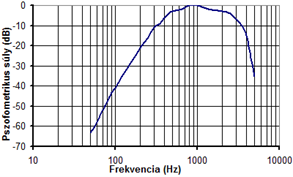
\includegraphics[width=0.4\textwidth]{frekvencia.png}
		\caption{A pszofometrikus súlytényező}
		\label{fig:frek}
	\end{figure}

	Minden esetben készítsünk neki egy képaláírást (\textit{\textcolor{bme}{Hivatkozások}} szalag, \textit{\textcolor{bme}{Feliratok}} csoport \textit{\textcolor{bme}{Képaláírás}} beszúrása).
	Itt válasszuk ki a megfelelő feliratot, ami értelemszerűen „ábra”.
	Sok ábra esetén érdemes lehet fejezetenként végezni az ábraszámozást, de erre egy 60-80 oldalas diplomaterv esetén is ritkán van szükség.
	\par
	A végén a képaláírás bekezdésén alkalmazzuk a Képaláírás stílust.
	Hivatkozást a \textit{\textcolor{bme}{Hivatkozás}} szalag \textit{\textcolor{bme}{Feliratok}} csoport \textit{\textcolor{bme}{Kereszthivatkozás}} parancsával lehet beszúrni (\ref{fig:frek}. ábra).
	Amennyiben folyó szövegben szeretnénk hivatkozni, a toldalékolásnál figyeljünk arra, hogy a \ref{fig:frek}. ábra címke záró a betűje nehezen változtatható á-ra.
	Ekkor a következő trükköt kell alkalmazni:
	\begin{enumerate}
		\item Szúrjuk be a szokásos kereszthivatkozást: \ref{fig:frek}. ábra.
		\item A hivatkozásra lépve váltuk át mezőkódokra: jobb gomb \textit{\textcolor{bme}{Mezőkódok - váltás}}, vagy Shift-F9 billentyűkombináció: \{REF\_Ref346714546\textbackslash h\}
		\item A záró kapcsos záró jel elé írjuk be, hogy „\textbackslash\# 0” (ez egy formátumsztring), tehát \\ \{REF\_Ref346714546\textbackslash h \textbackslash\# 0\}
		\item Váltsuk vissza a mezőkódot, s frissítsük a mező értékét (F9)!
		Az eredmény, hogy csak a számot tartalmazza a mező, ekkor már kézzel írhatjuk oda, hogy pl. ábrán.
		Ezzel megoldható például „látható az 5. és 6. ábrán”, vagy „a 9-11. ábra esetén” feliratok.
	\end{enumerate}

	\subsection{Táblázat}
	Táblázatot a \textit{\textcolor{bme}{Beszúrás}} szalag \textit{\textcolor{bme}{Táblázatok}} csoportjánál lehet beilleszteni.
	A formázása szintén automatikus, a \textit{\textcolor{bme}{Táblázateszközök}}/\textit{\textcolor{bme}{Tervezés}} szalag, \textit{\textcolor{bme}{Táblázatstílusok}} csoportból szabadon választható egy stílus.
	Függetlenül a választástól, a dokumentumon belüli egységes legyen a formázás.
	\begin{table}[h]
		\begin{center}
			\begin{tabular}{c|c|c|c}
				& állandó & órás & indító \\
				\hline
				$P_n$ [kW] & 1100 & 1130 & 1870 \\
				\hline
				$U_n$ [V] & 1100 & 1100 & 1100 \\
				\hline
				$I_n$ [A] & 1070 & 1100 & 1700 \\
			\end{tabular}
		\end{center}
		\caption{A motor névleges adatai \cite{BOOK:2}}
		\label{tab:motor}
    \end{table}
	Képaláírás az ábrákéhoz hasonlóan adható meg, hivatkozni is úgy kell.
	\subsection{Egyenlet}
	Egyenletet beszúrni a \textit{\textcolor{bme}{Beszúrás}} szalag \textit{\textcolor{bme}{Szimbólumok}} csoport \textit{\textcolor{bme}{Egyenlet}} parancsával lehet.
	(Ez a kompatibilitási csomaggal futó \textit{\textcolor{blue}{Office2003}}-ban és doc formátum esetén nem elérhető, ekkor a korábbi egyenletszerkesztőt kell használni.)
	Az új egyenletszerkesztő könnyedén használható, és utána a képletek részben vagy egészben másolhatók, amit a korábbinál nem lehetett megoldani.
	\par
	Az egyenletek rendezéséhez táblázatos módszert érdemes használni.
	Az egysoros táblázat első oszlopába kerül az egyenlet, a másodikba a számozás, ami ugyanúgy hivatkozható, mint a korábbi ábra illetve táblázat aláírás.
	A sablonban előkészítettünk egy ilyen egyenletet, melyet \textit{\textcolor{bme}{Beszúrás}} szalag Szimbólumok csoport \textit{\textcolor{bme}{Egyenlet}} parancsával, a megjelenő panel első sorában talál (Pitagorasz-tételt írja le, de értelemszerűen ez utána átírható az igényeknek megfelelően):
	\begin{equation}
		a^2 + b^2 = c^2 \label{eq:pit1}
	\end{equation}
	A magyarázathoz létezik az Egyenlet magyarázata stílus, amibe a tabulálás már be is van építve.
	Lásd a következő mintát:
	\begin{equation}
		f(t) = a_0 + \sum_{h=1}^\infty (a_h\cos(h\omega t)+ b_h \sin(h\omega t)) = c_0 + \sum_{h=1}^\infty(c_h\cos(h\omega t + \varphi_h)) \label{eq:2}
	\end{equation}
	ahol
	\begin{flalign*}
		&\omega = \frac{2\pi}{t} &&\text{azaz a körfrekvencia,} &&\\
		&c_0 &&\text{az egyenkomponens amplitúdója,} &&\\
		&c_h &&\text{a h. harmonikus amplitódja,} &&\\
		&\varphi_h &&\text{a h. harmonikus fázisszöge,} &&\\
		&h &&\text{a harmonikus rendszáma.} &&
	\end{flalign*}
	A magyarázat után az első bekezdést vissza kell állítani Normál stílusúra.
	A szövegközi hivatkozás hasonlóan kivitelezhető, mint az ábrák és táblázatok esetén volt látható.
	A legtöbb esetben érdemes megmagyarázni, hogy az egyenletben szereplő változók mit írnak le.
	A (\ref{eq:2}) ismerteti az inverz Fourier sorba fejtés képletét.
	\par
	Az egyenlet egy sorban, egyszerű tabulátorokkal is megoldható az Egyenlet stílus alkalmazásával.
	Ennek hátránya, hogy az egyenletben a törtek, illetve a felső és alsó indexek kicsinyítve jelennek meg: \\
	\begin{center}
	$f(t) = a_0 + \sum_{h=1}^\infty (a_h\cos(h\omega t)+ b_h \sin(h\omega t)) = c_0 + \sum_{h=1}^\infty(c_h\cos(h\omega t + \varphi_h)) \label{eq:3}$
	\end{center}

	\subsection{Kereszthivatkozások}
	Az eddigiekhez hasonlóan hivatkozhatunk fejezetekre is.
	Ebben az esetben is tegyük ezt dinamikusan, a \textit{\textcolor{bme}{Hivatkozás}} szalag \textit{\textcolor{bme}{Feliratok}} csoport \textit{\textcolor{bme}{Kereszthivatkozás}} paranccsal.
	Lehet hivatkozni minden esetben magára a címsorszámra, a címsorra és az oldalszámára is.
	A \ref{sec:3}.~fejezet címe: \nameref{sec:3}, a \pageref{sec:3}. oldalon kezdődik.
	Azért szükséges a dinamikus hivatkozás, mert ha módosul egy adat (pl. oldalszám, beszúrunk egy újabb fejezetet) akkor a hivatkozás helyén is automatikusan átíródik a tartalom.

	\subsection{Tizedesvessző, mértékegységek, ezres elválasztás}
	A Magyar Helyesírási Szabályzat szerint a tizedes operátor a vessző, és nem pedig a pont.
	Ez mind a képleteknél, mind a folyó szövegnél alkalmazandó.
	Amennyiben folyó szövegben mértékegységet is írunk a szám mögé, alkalmazzuk azt a szóköz típust, ami nem engedi a mértékegységet elválasztani a számtól, 400~kV (Ctrl+Shift+szóköz, és egy kis karika a jele).
	\par
	Ezres elválasztás alkalmazása nem szükséges (sőt, a szabályzat szerint 9999-ig helytelen).
	Amennyiben mégis ragaszkodunk hozzá, ismét alkalmazzuk a nem elválasztó szóközt, aminek a mérete fix.
	Semmiképpen ne használjunk erre pontot vagy vesszőt. 
	\par
	A Paksi Atomerőmű minden egyes blokkja 500~MW teljesítményű, ami átváltva 0,5~gigawattnak felel meg.
	Ez éppen 500000~kW vagy 500~000~000~W.

	\newpage
	\section{Irodalmi hivatkozások}
	\subsection{Stílustámogatás}
	Az Office is nyújt támogatás irodalmi hivatkozásokhoz (\textit{\textcolor{bme}{Hivatkozás}} szalag / \textit{\textcolor{bme}{Idézetek és irodalomjegyzék}} csoport), de egy-egy dolgozat esetében lehet, hogy célszerűbb egyszerű sorszámozást alkalmazni.
	Ez nem más, mint egy egyszerű sorszámozás, amit az Irodalomjegyzék stílus segít elő. Az irodalomjegyzékben tehát ez valójában egy sorszámozott lista.
	\par
	A szövegben erre a már megismert kereszthivatkozással hivatkozhatunk (számozott elem kategória).
	Hátránya a beépített irodalomjegyzékhez képest, hogy egyes esetekben nem, vagy rosszul frissül, előnye, hogy lényegesen egyszerűbb, s általában jól működik.
	A dolgozat beadásakor azonban érdemes megnézni a helyességét (akárcsak a többi hivatkozást is!).

	\subsection{Hol kell hivatkozni?}
	\begin{itemize}[label=\color{bme}$\bullet$]
		\item Mindenhol ahol szó szerint, idézőjelben veszünk át szövegeket.
		\item Minden ábra, illetve táblázat képaláírásában, amit máshonnét vettünk, s nem saját készítés vagy eredmény.
		(Ha saját készítés, de más források alapján, akkor is!)
		\item Irodalomkutatás esetén célszerűbb a fejezet elején (s nem a végén!) összefoglalni a felhasznált irodalmakat.
		Ha könnyebben szétválasztható, hogy egyes tartalmak honnét származtathatók, akkor az egyes bekezdések végére is tehető hivatkozás.
	\end{itemize}

	\subsection{Hogyan kell hivatkozni?}
	A szövegben egyszerű számmal hivatkozunk, nincs szükséges külön szó alkalmazására.
	Pl. téves azt írni, hogy, ld. \cite{BOOK:2} forrás. Ehelyett egyszerűen írjunk annyit, hogy \cite{BOOK:2}.
	\newpage
	\bibliography{Temalab_sablon} 
	\bibliographystyle{unsrt}
	\newpage




	\setcounter{page}{1}
	\setcounter{section}{0}
	\section*{Függelék}
	\addcontentsline{toc}{section}{Függelék}
	A függelék előtt kell egy szakasztörés, mert ezzel ebben a szakaszban új oldalszámozás kezdődik.

	\titleformat{\section}{\color{fuggelekkek}\large\bfseries}{F\thesection\;}{0em}{}[\vspace{-3ex}\rule{\textwidth}{0.5pt}]

	\titleformat{\subsection}{\color{fuggelekkek}\large}{F\thesubsection\;}{0em}{}[\vspace{-3ex}\rule{\textwidth}{0.5pt}]

	\titleformat{\subsubsection}{\color{fuggelekkek}}{F\thesubsubsection\;}{0em}{}[\vspace{-3ex}\rule{\textwidth}{0.5pt}]

	\section{Első függelék címsor}
	Függelék beszúrása esetén ugyanazok a teendők, mint a fő résznél.
	Annyi a különbség, hogy itt a FCímsor stílusokat kell keresni.
	Függelék csak ettől az oldaltól kezdve szúrható be!
	\subsection{Első függelék alcím}
	Itt is alkalmazhatunk további szinteket, ide is szúrhatunk be ábrákat, táblázatokat, egyenleteket ugyanúgy, mint a korábbi részeknél.
	\subsubsection{Első függelék al-alcím}
	Teszt sor.
\end{document}
